\section{Styles}
\subsection{Schriftart}
Durch den Common-Component \textbf{Text} können wir jedem Textfeld in der App eine einheitliche Schriftart
geben. Ich entschied mich für die Font Poppins \cite{poppins}.

\subsection{Farbwerte}
Alle Farben, die man in der App sehen kann, wurden in der Datei \textbf{Colors.js} in
\textbf{root/styles} festgelegt. So muss nicht, sollte sich das Design ändern müssen, in jedem
StyleSheet jede Farbe einzeln getauscht werden.

Die Hauptfarbe der App ist der wunderschöne Grünton Jade (\#00A86B), welchen ich durch die Webseite
color-name.com \cite{colorName} fand. Die Webseite MyColor.Space \cite{myColorSpace} erzeugt anhand
einer Farbe mehrere andere Farben, die gut dazu passen.

\subsection{Icons}
Die Bibliothek \textbf{react-native-vector-icons} \cite{reactNativeVectorIcons} war eine große Hilfe
bei der Erstellung des Designs, Icons sind nämlich der perfekte Weg, um Informationen auf wenig Platz
darzustellen, z.B. welche Funktion ein Knopf hat. Ich habe stets darauf geachtet diverse Icons von
verschiedenen Anbietern in die App einzubauen. Hauptsächlich verwende ich die
\textbf{MaterialCommunityIcons}, eine große Sammlung von Icons orientiert am Material Design, einer
Designsprache entwickelt von Google.

\newpage
\subsection{FlashMessage}
\begin{code}[htp]
\begin{lstlisting}[firstnumber=1,language=JavaScript, style=JSX]
const App = () => (
  ...
  <FlashMessage position="top" />
  ...
);

export default App;
\end{lstlisting}
\caption{React Component - FlashMessage-Komponente in root/App.js}
\end{code}

Die Komponente FlashMessage ist für Mitteilungen über Geschehnisse in der App zuständig, z.B.
Login fehlgeschlagen oder Login erfolgreich.

\begin{figure}[H]
  \begin{center}
    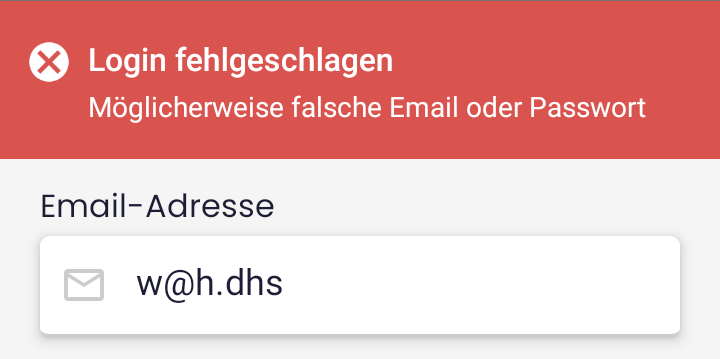
\includegraphics[width=0.5\textwidth]{Mobile/Auth/failed.png}
    \caption{Login-Informationen falsch}
  \end{center}
\end{figure}

\begin{figure}[H]
  \begin{center}
    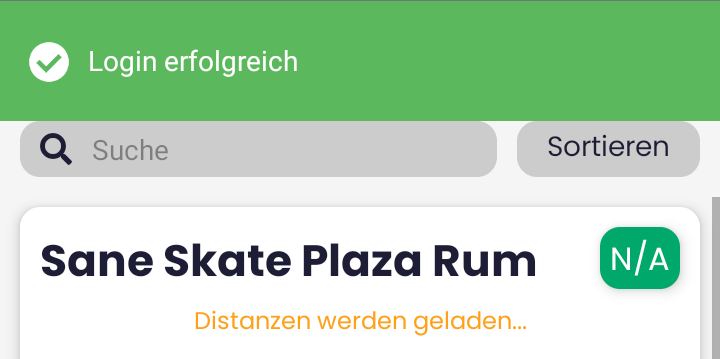
\includegraphics[width=0.5\textwidth]{Mobile/Auth/granted.png}
    \caption{Login-Informationen richtig}
  \end{center}
\end{figure}